\documentclass[12pt]{report}
\usepackage[utf8]{inputenc}
\usepackage[russian]{babel}
%\usepackage[14pt]{extsizes}
\usepackage{listings}
\usepackage{amsmath}
\usepackage[justification=centering]{caption}

\lstdefinelanguage{Kotlin}{
  comment=[l]{//},
  commentstyle={\color{gray}\ttfamily},
  emph={delegate, filter, first, firstOrNull, forEach, lazy, map, mapNotNull, println, return@},
  emphstyle={\color{orange}},
  identifierstyle=\color{black},
  keywords={abstract, actual, as, as?, break, by, class, companion, continue, data, do, dynamic, else, enum, expect, false, final, for, fun, get, if, import, in, interface, internal, is, null, object, override, package, private, public, return, set, super, suspend, this, throw, true, try, typealias, val, var, vararg, when, where, while},
  keywordstyle={\color{blue}\bfseries},
  morecomment=[s]{/*}{*/},
  morestring=[b]",
  morestring=[s]{"""*}{*"""},
  ndkeywords={@Deprecated, @JvmField, @JvmName, @JvmOverloads, @JvmStatic, @JvmSynthetic, Array, Byte, Double, Float, Int, Integer, Iterable, Long, Runnable, Short, String},
  ndkeywordstyle={\color{orange}\bfseries},
  sensitive=true,
  stringstyle={\color{green}\ttfamily},
}

% Для листинга кода:
\lstset{ %
language=Kotlin,                 % выбор языка для подсветки (здесь это С)
basicstyle=\footnotesize\sffamily, % размер и начертание шрифта для подсветки кода
numbers=left,               % где поставить нумерацию строк (слева\справа)
numberstyle=\tiny,           % размер шрифта для номеров строк
stepnumber=1,                   % размер шага между двумя номерами строк
numbersep=5pt,                % как далеко отстоят номера строк от подсвечиваемого кода
showspaces=false,            % показывать или нет пробелы специальными отступами
showstringspaces=false,      % показывать или нет пробелы в строках
showtabs=false,             % показывать или нет табуляцию в строках
frame=single,              % рисовать рамку вокруг кода
tabsize=2,                 % размер табуляции по умолчанию равен 2 пробелам
captionpos=t,              % позиция заголовка вверху [t] или внизу [b] 
breaklines=true,           % автоматически переносить строки (да\нет)
breakatwhitespace=false, % переносить строки только если есть пробел
escapeinside={\#*}{*)}   % если нужно добавить комментарии в коде
}

\usepackage{hyperref}
\hypersetup{
    linktoc=all,     %set to all if you want both sections and subsections linked
    linkcolor=blue,  %choose some color if you want links to stand out
}

% Для измененных титулов глав:
\usepackage{titlesec, blindtext, color} % подключаем нужные пакеты
\definecolor{gray75}{gray}{0.75} % определяем цвет
\newcommand{\hsp}{\hspace{20pt}} % длина линии в 20pt
% titleformat определяет стиль
\titleformat{\chapter}[hang]{\Huge\bfseries}{\thechapter\hsp\textcolor{gray75}{|}\hsp}{0pt}{\Huge\bfseries}


\begin{filecontents}{brut.dat}
1000 235190.6
1500 298602.5
2000 365434.6
2500 441495.8
3000 499925.5
3500 577187.2
\end{filecontents}


\begin{filecontents}{bin.dat}
1000 228380.5
1500 313386.9
2000 390250.1
2500 484867.6
3000 568735.6
3500 656122.9
\end{filecontents}

\begin{filecontents}{mod.dat}
1000 229931.4
1500 313806.5
2000 400287.4
2500 487058.9
3000 579073.5
3500 676655.8
\end{filecontents}


\begin{filecontents}{brutMax.dat}
1000 5213669
1500 5421492
2000 5676778
2500 5898154
3000 7868180
3500 6189138
\end{filecontents}


\begin{filecontents}{binMax.dat}
1000 1934776
1500 1954133
2000 1973740
2500 1489540
3000 2063660
3500 1748799
\end{filecontents}

\begin{filecontents}{modMax.dat}
1000 1914085
1500 734985
2000 1043134
2500 1826962
3000 2258136
3500 2547382
\end{filecontents}


% plot
\usepackage{pgfplots}
\usepackage{filecontents}
\usetikzlibrary{datavisualization}
\usetikzlibrary{datavisualization.formats.functions}

\begin{document}
\begin{titlepage}
	\fontsize{12pt}{12pt}\selectfont
	\noindent \begin{minipage}{0.15\textwidth}
		
\includegraphics[width=\linewidth]{inc/img/b_logo.jpg}
	\end{minipage}
	\noindent\begin{minipage}{0.9\textwidth}\centering
		\textbf{Министерство науки и высшего образования Российской Федерации}\\
		\textbf{Федеральное государственное бюджетное образовательное учреждение высшего образования}\\
		\textbf{«Московский государственный технический университет имени Н.Э.~Баумана}\\
		\textbf{(национальный исследовательский университет)»}\\
		\textbf{(МГТУ им. Н.Э.~Баумана)}
	\end{minipage}
	
	\noindent\rule{15cm}{3pt}
	\newline\newline
	\noindent ФАКУЛЬТЕТ \underline{~~~~~~~~~~~~~~~~«Информатика и системы управления»~~~~~~~~~~~~~~~~} \newline\newline
	\noindent КАФЕДРА \underline{«Программное обеспечение ЭВМ и информационные технологии»}\newline\newline\newline\newline\newline\newline\newline
	
	
	\begin{center}
		\Large\textbf{Отчет по лабораторной работе №7 по курсу "Анализ алгоритмов"}\newline
	\end{center}
	
	\noindent\textbf{Тема} \underline{Поиск в словаре}\newline\newline\newline
	\noindent\textbf{Студент} \underline{Якуба Д. В.}\newline\newline
	\noindent\textbf{Группа} \underline{ИУ7-53Б}\newline\newline
	\noindent\textbf{Оценка (баллы)} \underline{~~~~~~~~~~~~~~~~~~~}\newline\newline
	\noindent\textbf{Преподаватели} \underline{Волкова Л.Л., Строганов Ю.В.}\newline
	
	\begin{center}
		\vfill
		Москва~---~\the\year
		~г.
	\end{center}
\end{titlepage}

\setcounter{page}{2}

\tableofcontents

\newpage
\chapter*{Введение}
\addcontentsline{toc}{chapter}{Введение}
\section*{Цель лабораторной работы}
Реализация алгоритмов поиска по словарю: перебором, бинарным поиском и с применением частотного анализа.
\section*{Задачи лабораторной работы}
\begin{enumerate}
\item[1)] изучить алгоритм поиска по словарю полным перебором;
\item[2)] изучить алгоритм бинарного поиска по словарю;
\item[3)] изучить алгоритм поиска по словарю с применением частотного анализа;
\item[4)] протестировать реализованные алгоритмы;
\item[5)] провести анализ временных характеристик реализованных алгоритмов;
\item[6)] подготовить отчёт по проведенной работе.
\end{enumerate}

\chapter{Аналитическая часть}
В данном разделе описаны определение словаря как структуры данных, а также алгоритмы поиска по словарю.

\section{Словарь}
Словарь (ассоциативный массив)\cite{NIST} — это абстрактный тип данных, хранящий пары вида «(ключ, значение)» и поддерживающий операции добавления пары, а также поиска и удаления пары по ключу:
\begin{itemize}
\item $INSERT(\textit{ключ, значение})$;
\item $FIND(\textit{ключ})$;
\item $REMOVE(\textit{ключ})$.
\end{itemize}

Предполагается, что все ключи в словаре являются уникальными.

В паре $(\textit{ключ, значение})$ $\textit{значение}$ называется значением, ассоциированным с ключом.

Операция $FIND(\textit{ключ})$ возвращает значение, ассоциированное с заданным ключом, или некоторый специальный объект, означающий, что значения, ассоциированного с заданным ключом, нет. Две другие операции ничего не возвращают (за исключением, возможно, информации о том, успешно ли была выполнена данная операция).

\section{Алгоритм поиска по словарю полным перебором}
Алгоритм полного перебора \cite{AI} — это алгоритм разрешения математических задач, который можно отнести к классу способов нахождения решения рассмотрением всех возможных вариантов.

Для решения поставленной задачи поиска с использованием метода полного перебора потребуется последовательно просматривать каждую запись в словаре. В том случае, если у рассматриваемой пары ключ совпадает с искомым - алгоритм завершает свою работу, задача выполнена.

Трудоёмкость алгоритма зависит от того, присутствует ли искомый ключ в словаре, и, если присутствует - насколько он далеко от начала массива ключей.

При решении задачи возможно возникновение $(N + 1)$ случаев, где $N$ - это количество записей в словаре: ключ не найден и $N$ возможных случаев расположения ключа в словаре.

Лучшим случаем для рассматриваемого алгоритма будет факт того, что искомый ключ был обнаружен за одно сравнение (то есть ключ находится в начале словаря).

Худший случай наступает при следующих стечениях обстоятельств:
\begin{itemize}
\item элемент не был найден за $N$ сравнений;
\item ключ был обнаружен на последнем сравнении.
\end{itemize}

Пусть на старте алгоритм поиска затрачивает $k_0$ операций, а при каждом сравнении $k_1$ операций. Тогда в лучшем случае потребуется $k_0 + k_1$ операций; в случае, если ключ был найден на втором сравнении - потребуется $k_0 + 2k_1$ операций; в случае нахождения ключа на последней позиции или его отсутствия в словаре - потребуется $k_0 + Nk_1$ операций.

Средняя трудоёмкость алгоритма может быть рассчитана как математическое ожидание по формуле \ref{MX} ($\Omega$ - множество всех возможных исходов).

\label{MX}
\begin{multline}
        \sum\limits_{i \in \Omega} p_i \cdot f_i = (k_0 + k_1) \cdot \frac{1}{N + 1} + (k_0 + 2 \cdot k_1) \cdot \frac{1}{N+1} + (k_0 + 3 \cdot k_1) \cdot \frac{1}{N + 1} + \\+ (k_0 + Nk_1)\frac{1}{N + 1} + (k_0 + N \cdot k_1) \cdot \frac{1}{N + 1} = \\= k_0\frac{N+1}{N+1}+k_1+\frac{1 + 2 + \cdots + N + N}{N + 1} = k_0 + k_1 \cdot \left(\frac{N}{N + 1} + \frac{N}{2}\right) =\\= k_0 + k_1 \cdot \left(1 + \frac{N}{2} - \frac{1}{N + 1}\right)
\end{multline}

\section{Алгоритм бинарного поиска по словарю}
При двоичном поиске обход можно представить деревом, поэтому трудоёмкость в худшем случае составит $\log_2N$ (спуск по двоичному дереву от корня до листа). Скорость роста функции $\log_2N$ меньше, чем у $N$.

\section{Частотный анализ}
Некоторый алгоритм на получает словарь и по нему составляется частотный анализ:
\begin{itemize}
\item по частоте использования ключа на реальных данных;
\item по частоте появления в выборке первого символа ключа (или его остатка от деления на некоторое значение в случае чисел).
\end{itemize}

По предоставленному отчёту словарь разбивается на сегменты. В каждом сегменте находятся элементы с некоторым, определённым анализатором, признаком.

Сегменты также могут быть упорядочены, например, по размеру сегмента, если множество исходов обращений к сегменту имеет высокую дисперсию.

Вероятность обращения к определенному сегменту равна сумме вероятностей обращений к его ключам (формула \ref{Pi}, где $P_i$ - вероятность обращения к $i$-ому сегменту, $p_j$ - вероятность обращения к $j$-ому элементу, который принадлежит $i$-ому сегменту).

\begin{equation}
\label{Pi}
P_i = \sum_{j}p_j
\end{equation}

Если обращения ко всем ключам равновероятны, то можно заменить сумму на произведение (формула \ref{PiProd}, где $N$ - количество элементов в $i$-ом сегменте, а $p$ - вероятность обращения к произвольному ключу).

\begin{equation}
\label{PiProd}
P_i = N \cdot p
\end{equation}

Ключи в сегментах также упорядочиваются для проведения бинарного поиска.

Как итог, сначала с помощью бинарного поиска выбирается требующийся сегмент. В найденном сегменте с помощью алгоритма бинарного поиска обнаруживается требующийся ключ. Средняя трудоёмкость представленного алгоритма действий будет определяться формулой \ref{ohgod}, где $M$ - количество сегментов.

\begin{equation}
    \label{ohgod}
    f_cp = \sum_{i \in [1, M]}{\left(f_{\text{выбора i-го сегмента}} + f_{\text{ср. поиска в i-м сегменте}}\right)} \cdot p_i
\end{equation}


\section*{Вывод}
Были рассмотрены определение словаря как структуры данных, а также алгоритмы поиска по словарю и оптимизации поиска.

В данной работе стоит задача реализации трёх рассмотренных алгоритмов поиска.

\chapter{Конструкторская часть}
В данном разделе представлены структура записей в словаре, а также схемы алгоритма поиска по словарю полным перебором, с использованием бинарного поиска, а также с использованием сегментирования и частотного анализа.
\section{Структура записи в словаре}
Каждая запись в словаре описана парой вида $(ID_{\textit{студента}} : \textit{Название курсового проекта})$.

\section{Схема алгоритма поиска по словарю полным перебором}
Схема алгоритма поиска полным перебором предоставлена на рисунке \ref{img:brutAlg}.

\begin{figure}
\begin{center}
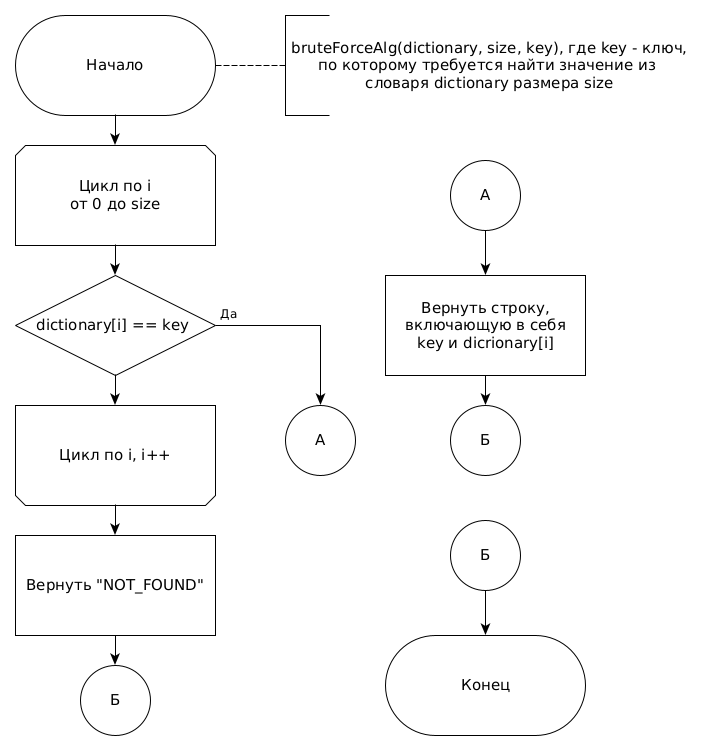
\includegraphics[scale=0.4]{inc/img/brutAlg.png}
\captionsetup{justification=centering}
	\caption{Схема алгоритма поиска полным перебором.}
	\label{img:brutAlg}	
\end{center}
\end{figure}

\section{Схема алгоритма бинарного поиска по словарю}
Схема алгоритма бинарного поиска по словарю предоставлена на рисунке \ref{img:binAlg}.

\begin{figure}
\begin{center}
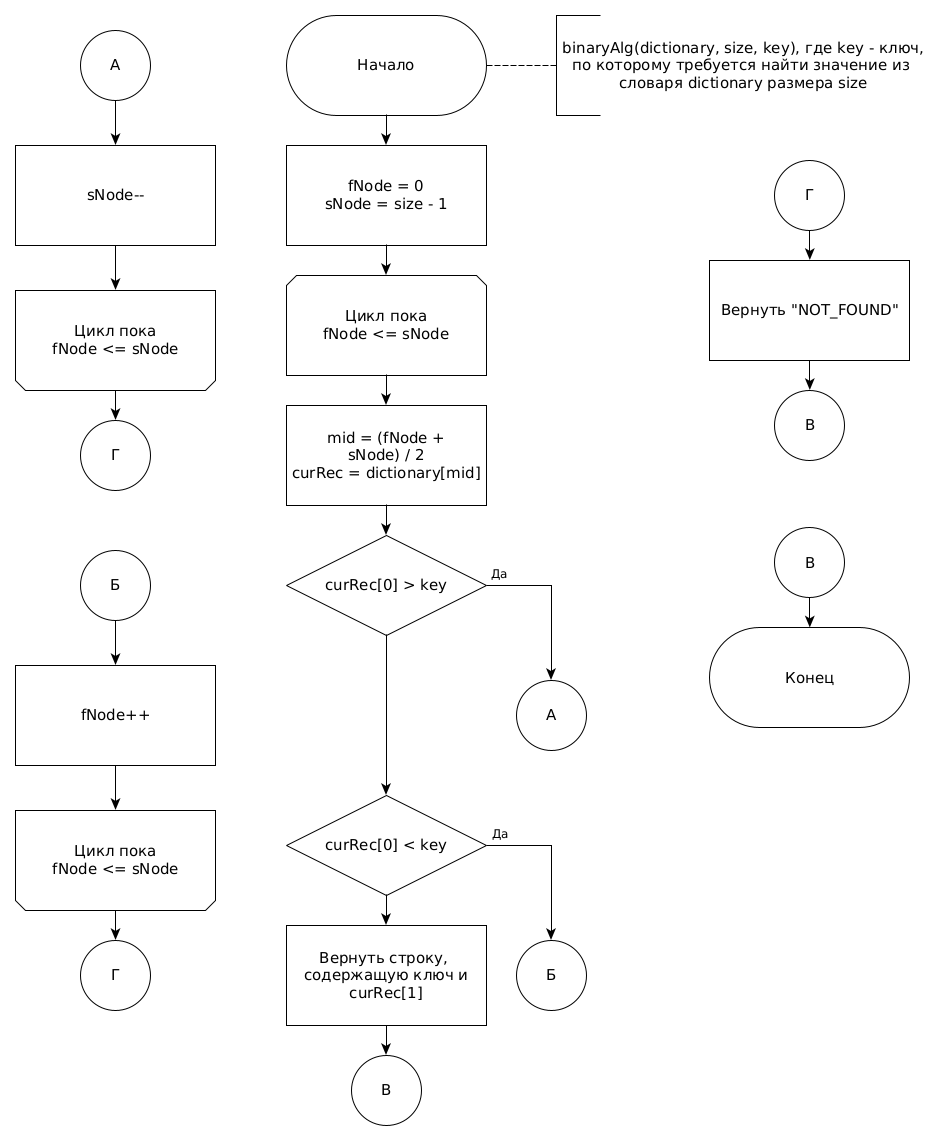
\includegraphics[scale=0.4]{inc/img/binAlg.png}
\captionsetup{justification=centering}
	\caption{Схема алгоритма бинарного поиска по словарю.}
	\label{img:binAlg}	
\end{center}
\end{figure}

\section{Схема алгоритма поиска по словарю с использованием разбиения на сегменты}
Схема алгоритма бинарного поиска по словарю с использование разбиения на сегменты предоставлена на рисунке \ref{img:binAlgUpd}.

\begin{figure}
\begin{center}
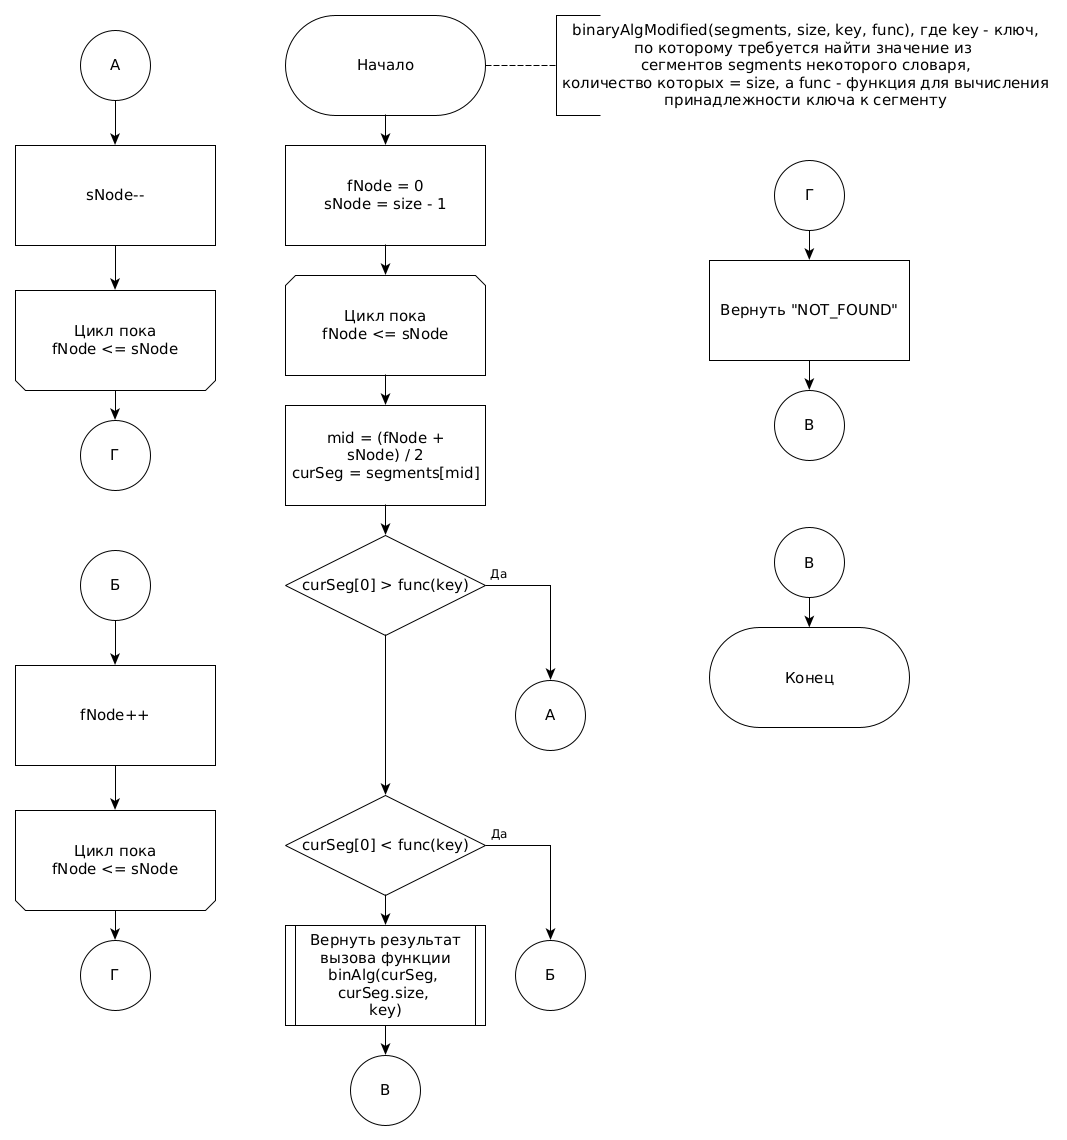
\includegraphics[scale=0.4]{inc/img/binAlgUpd.png}
\captionsetup{justification=centering}
	\caption{Схема алгоритма бинарного поиска по словарю с сегментированием.}
	\label{img:binAlgUpd}	
\end{center}
\end{figure}

\section*{Вывод}
Были представлены структура записей в словаре, а также схемы алгоритма поиска по словарю полным перебором, с использованием бинарного поиска, а также с использованием сегментирования и частотного анализа.

\chapter{Технологическая часть}
В данном разделе приведены требования к программному обеспечению, средства реализации программного обеспечения, а также листинг кода.

\section{Требования к программному обеспечению}
\begin{itemize}
\item входные данные - словарь и искомый ключ;
\item выходные данные - значение, соответствующее ключу в словаре, если он в нём присутствует, иначе - строка $"NOT\_FOUND"$.
\end{itemize}

\section{Средства реализации программного обеспечения}
При написании программного продукта был задействован язык программирования Kotlin \cite{Kotlin}.

Данный выбор обусловлен следующими факторами:
\begin{itemize}
\item Возможность портирования алгоритмов для работы с Android;
\item Большое количество справочной литературы, связанной с ЯП Java.
\end{itemize}

Для тестирования производительности реализаций алгоритмов использовалась утилита measureTimedValue.

При написании программного продукта использовалась среда разработки IntelliJ IDEA \cite{IntelliJ}.

Данный выбор обусловлен тем, что язык программирования Kotlin - это разработка компании JetBrains, поставляющей данную среду разработки.

Для написания утилиты, генерирующей данные для словаря, использовался ЯП Python\cite{Python}. 
Данный выбор обусловлен простотой языка.

Для генерации значений в словаре использовалась библиотека Faker \cite{Faker} для ЯП Python.

\section{Листинг кода}
В листинге \ref{list:Dict} предоставлены реализации рассматриваемых алгоритмов.
\begin{lstlisting}[caption=Реализации рассматриваемых алгоритмов поиска,
label={list:Dict}]
class Dictionary
{
    private val NOT_FOUND = "NOT_FOUND"

    private val dictionary: MutableList<Pair<Int, String>> = mutableListOf()
    private val segmentedDictionary: MutableList<Pair<Int, MutableList<Pair<Int, String>>>> = mutableListOf()

    private val secretFunc: (Int) -> (Int) = { it % 100 }

    fun isEmpty() : Boolean
    {
        return dictionary.isEmpty()
    }

    fun fullByFile(filePath: String)
    {
        val reader = Files.newBufferedReader(Paths.get(filePath))
        val parser = CSVParser(reader, CSVFormat.DEFAULT.withDelimiter(';'))

        for (curRecord in parser)
            dictionary.add(Pair(curRecord[0].toInt(), curRecord[1]))

        if (!parser.isClosed)
            parser.close()

        dictionary.shuffle()
    }

    fun getValueByBrutForce(key: Int) : String
    {
        for (curIndex in 0 until dictionary.size)
        {
            if (dictionary[curIndex].first == key)
                return "{ %d : %s }".format(key, dictionary[curIndex].second)
        }
        return NOT_FOUND
    }

    fun sortForBinarySearch(dictionary_: MutableList<Pair<Int, String>> = this.dictionary)
    {
        dictionary_.sortBy { it.first }
    }

    fun getValueByBinarySearch(key: Int, dictionary_: MutableList<Pair<Int, String>> = this.dictionary) : String
    {
        var firstNode = 0
        var secondNode = dictionary_.size - 1
        while (firstNode <= secondNode)
        {
            val middle = (firstNode + secondNode) / 2
            val curRecordID = dictionary_[middle]

            when
            {
                curRecordID.first > key -> secondNode--
                curRecordID.first < key -> firstNode++
                else -> return "{ %d : %s }".format(key, curRecordID.second)
            }
        }

        return NOT_FOUND
    }

    fun createSegmentedDictionary()
    {
        for (i in 0 until 100)
            segmentedDictionary.add(Pair(i, dictionary.filter { secretFunc(it.first) == i }.toMutableList()))

        segmentedDictionary.forEach { segment -> segment.second.sortBy { it.first } }
        segmentedDictionary.sortBy { it.second.size }
    }

    fun getValueBySegmentedAndBinaryModified(key: Int) : String
    {
        if (segmentedDictionary.isEmpty())
            return "No segmented array."

        var firstNode = 0
        var secondNode = segmentedDictionary.size - 1
        while (firstNode <= secondNode)
        {
            val middle = (firstNode + secondNode) / 2
            val curSegment = segmentedDictionary[middle]

            when
            {
                curSegment.first > secretFunc(key) -> secondNode--
                curSegment.first < secretFunc(key) -> firstNode++
                else -> return getValueByBinarySearch(key, curSegment.second)
            }
        }

        return NOT_FOUND
    }

    fun print()
    {
        for (i in dictionary)
            println(i)
    }
}
\end{lstlisting}

\section{Тестирование программного продукта}
В таблице~\ref{tabular:test_rec} приведены тесты для функций поиска значений в словаре по ключу. Тесты пройдены успешно.

\begin{table}[h!]
	\begin{center}
	
	\caption{\label{tabular:test_rec} Тестирование функций}
		\begin{tabular}{c@{\hspace{7mm}}c@{\hspace{7mm}}}
			\hline
			Ключ & Ожидаемый результат \\ \hline
			\vspace{4mm}
			 666&
			 Эксплуатация богатых парадигм\\
			\vspace{2mm}
			\vspace{2mm}
			 22&
			 Ускорение сетевых схем\\
			\vspace{2mm}
			\vspace{2mm}
			 1001&
			 $NOT\_FOUND$\\
			\vspace{2mm}
			\vspace{2mm}
			 -1&
			 $NOT\_FOUND$\\
		\end{tabular}
	\end{center}
\end{table}
\newpage

\section*{Вывод}
Спроектированные алгоритмы были реализованы и протестированы.

\chapter{Исследовательская часть}
\section{Технические характеристики}
Технические характеристики ЭВМ, на котором выполнялись исследования:
\begin{itemize}
\item ОС: Manjaro Linux 20.1.1 Mikah;
\item Оперативная память: 16 Гб;
\item Процессор: Intel Core i7-10510U.
\end{itemize}

При проведении замеров времени ноутбук был подключен к сети электропитания.

\section{Пример работы программного обеспечения}
На рисунках \ref{img:example1}, \ref{img:example2} приведены примеры работы программы.

\begin{figure}[!ht]
\begin{center}
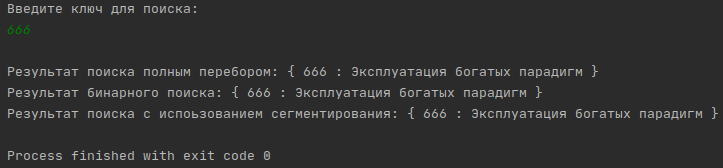
\includegraphics[scale=0.7]{inc/img/example1.png}
\captionsetup{justification=centering}
	\caption{Пример работы ПО.}
	\label{img:example1}	
\end{center}
\end{figure}

\begin{figure}[!ht]
\begin{center}
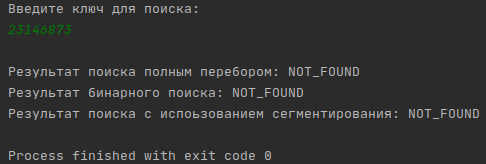
\includegraphics[scale=1.1]{inc/img/example2.png}
\captionsetup{justification=centering}
	\caption{Пример работы ПО.}
	\label{img:example2}	
\end{center}
\end{figure}

\newpage
\section{Время выполнения алгоритмов}
Алгоритм тестировался на данных, сгенерированных случайным образом.

В таблицах \ref{time1}-\ref{time3} предоставлены результаты проведённых замеров времени. $t_{cp}$- среднее время работы алгоритма, $t_{max}$ - максимально зафиксированное время работы, $t_{min}$ - минимально зафиксированное время работы алгоритма. Время замерялось для поиска каждого элемента в словаре, включая поиск по ключу, отсутствующему в словаре.

На рисунках \ref{timeRes1}, \ref{timeRes2} приведены графики зависимости среднего и максимального времени исполнения алгоритмов от количества записей в словаре.

\begin{table}[h]
	\begin{center}
		\caption{\label{time1} Замеры времени для поиска полным перебором}
		\begin{tabular}{|c | c | c | c|} 
 			\hline
			Количество элементов словаря & $t_{cp}$, нс & $t_{max}$, нс & $t_{min}$, нс\\ [0.5ex] 
 			\hline\hline
 			1000 & 235190.6 & 5213669 & 52750\\
 			\hline
 			1500 & 298602.5 & 5421492 & 52434\\
 			\hline
 			2000 & 365434.6 & 5676778 & 51980\\
 			\hline
 			2500 & 441495.8 & 5898154 & 51881\\
 			\hline
 			3000 & 499925.5 & 7868180 & 52996\\
 			\hline
 			3500 & 577187.2 & 6189138 & 52074\\
 			\hline
			\end{tabular}
	\end{center}
\end{table}

\begin{table}[h]
	\begin{center}
		\caption{\label{time2} Замеры времени для бинарного поиска}
		\begin{tabular}{|c | c | c | c|} 
 			\hline
			Количество элементов словаря & $t_{cp}$, нс & $t_{max}$, нс & $t_{min}$, нс\\ [0.5ex] 
 			\hline\hline
 			1000 & 228380.5 & 1934776 & 52675\\
 			\hline
 			1500 & 313386.9 & 1954133 & 52689\\
 			\hline
 			2000 & 390250.1 & 1973740 & 52435\\
 			\hline
 			2500 & 484867.6 & 1489540 & 52461\\
 			\hline
 			3000 & 568735.6 & 2063660 & 52997\\
 			\hline
 			3500 & 656122.9 & 1748799 & 52638\\
 			\hline
			\end{tabular}
	\end{center}
\end{table}


\begin{table}[h]
	\begin{center}
		\caption{\label{time3} Замеры времени для модифицированного поиска}
		\begin{tabular}{|c | c | c | c|} 
 			\hline
			Количество элементов словаря & $t_{cp}$, нс & $t_{max}$, нс & $t_{min}$, нс\\ [0.5ex] 
 			\hline\hline
 			1000 & 229931.4 & 1914085 & 52949\\
 			\hline
 			1500 & 313806.5 & 734985 & 52377\\
 			\hline
 			2000 & 400287.4 & 1043134 & 52414\\
 			\hline
 			2500 & 487058.9 & 1826962 & 52996\\
 			\hline
 			3000 & 579073.5 & 2258136 & 53335\\
 			\hline
 			3500 & 676655.8 & 2547382 & 52933\\
 			\hline
			\end{tabular}
	\end{center}
\end{table}

\begin{figure}[h]
\begin{center}
	\begin{tikzpicture}
	
\begin{axis}[
  		  	axis lines = left,
  		  	xlabel = количество записей,
  		  	ylabel = {время, нс},
			legend pos=north west,
			ymajorgrids=true
		] 
		\addplot[color=red] table[x index=0, y index=1] {brut.dat};
 		\addplot[color=blue, mark=square] table[x index=0, y index=1] {bin.dat};
		\addplot[color=green, mark=square] table[x index=0, y index=1] {mod.dat};

		\addlegendentry{Полный перебор}
		\addlegendentry{Бинарный поиск}
		\addlegendentry{Сегментированный алг.}
		\end{axis}
	\end{tikzpicture}
	\captionsetup{justification=centering}
	\caption{Зависимость среднего времени работы от количества записей в словаре}
	\label{timeRes1}
	\end{center}
\end{figure}

\begin{figure}[h]
\begin{center}
	\begin{tikzpicture}
	
\begin{axis}[
  		  	axis lines = left,
  		  	xlabel = количество записей,
  		  	ylabel = {время, нс},
			legend pos=north west,
			ymajorgrids=true
		] 
		\addplot[color=red] table[x index=0, y index=1] {brutMax.dat};
 		\addplot[color=blue, mark=square] table[x index=0, y index=1] {binMax.dat};
		\addplot[color=green, mark=square] table[x index=0, y index=1] {modMax.dat};

		\addlegendentry{Полный перебор}
		\addlegendentry{Бинарный поиск}
		\addlegendentry{Сегментированный алг.}
		\end{axis}
	\end{tikzpicture}
	\captionsetup{justification=centering}
	\caption{Зависимость максимального времени работы от количества записей в словаре}
	\label{timeRes2}
	\end{center}
\end{figure}

\newpage

\section*{Вывод}
Из предоставленной таблицы видно, что, как и ожидалось, минимальное время нахождение значения по ключу во всех трёх алгоритма приблизительно равны некоторой константе.

Из графика, предоставленного на рисунке \ref{timeRes1} видно, что, так или иначе, алгоритм полного перебора в текущей реализации на всей прямой работает несколько быстрее двух других алгоритмов. На начальных значениях в 1000 записей полный перебор показывает себя хуже на $\approx 3\%$, чем алгоритм бинарного поиска, и на $\approx 2\%$ хуже, чем модифицированный алгоритм. На остальных значениях размера словаря этот алгоритм будет быстрее бинарного поиска в среднем на $\approx 9800$ наносекунд. Относительно модифицированного алгоритма поиска это значение вырастает до $\approx 16603$ наносекунд. Такое странное поведение скорости исполнения обусловлено выполнением кода на виртуальной машине Java \cite{JVM} без оптимизаций, то есть в режиме интерпретации строк кода. Так как алгоритм полного перебора занимает много меньше операций, он и работает в среднем быстрее остальных, более ёмких алгоритмов. Это же объясняет факт преобладания по скорости алгоритма бинарного поиска над сегментированным алгоритмом, так как сегментированный алгоритм, грубо говоря, включает в себя два алгоритма бинарного поиска.

Из графика, предоставленного на рисунке \ref{timeRes2} видно, что предоставленные алгоритмы бинарного поиска и сегментированный алгоритм позволяют снизить максимальное время поиска значения по ключу. Для алгоритма бинарного поиска разница с алгоритмом полного перебора на 1500 записях словаря составила $\approx 277\%$. Для модифицированного алгоритма разница с алгоритмом полного перебора на 1500 записях словаря составила $\approx 738\%$.

\chapter*{Заключение}
\addcontentsline{toc}{chapter}{Заключение}
В ходе выполнения лабораторной работы была выполнена цель и следующие задачи:
\begin{enumerate}
\item[1)] был изучен алгоритм поиска по словарю полным перебором;
\item[2)] был изучен алгоритм бинарного поиска по словарю;
\item[3)] был изучен алгоритм поиска по словарю с применением частотного анализа;
\item[4)] реализованные алгоритмы были протестированы;
\item[5)] был проведён анализ временных характеристик реализованных алгоритмов;
\item[6)] был подготовлен отчёт по проведенной работе.
\end{enumerate}

Исследования показали, что:
\begin{itemize}
\item предоставленные алгоритмы бинарного поиска и сегментированный алгоритм позволяют снизить максимальное время поиска значения по ключу;
\item алгоритм полного перебора в текущей реализации работает быстрее двух других алгоритмов, начиная с размерности словаря в 1500 записей;
\item алгоритм полного перебора при 3500 записях в словаре работает быстрее алгоритма бинарного поиска на $\approx 14\%$;
\item алгоритм полного перебора при 3500 записях в словаре работает быстрее модифицированного алгоритма поиска на $\approx 17\%$;
\item алгоритм бинарного поиска на 3500 записях в словаре работает быстрее модифицированного алгоритма на $\approx 3\%$.
\end{itemize}

\addcontentsline{toc}{chapter}{Литература}
\bibliographystyle{utf8gost705u}  % стилевой файл для оформления по ГОСТу
\bibliography{biblio.bib}          % имя библиографической базы (bib-файла)


\end{document} 
